
%% conf_paper.tex

\documentclass[conference]{IEEEtran}
% Add the compsoc option for Computer Society conferences.
%
% If IEEEtran.cls has not been installed into the LaTeX system files,
% manually specify the path to it like:
% \documentclass[conference]{../sty/IEEEtran}


% *** GRAPHICS RELATED PACKAGES ***
%
\ifCLASSINFOpdf
   \usepackage[pdftex]{graphicx}
  % declare the path(s) where your graphic files are
   \graphicspath{{../pdf/}{../jpeg/}}
  % and their extensions so you won't have to specify these with
  % every instance of \includegraphics
   \DeclareGraphicsExtensions{.pdf,.jpeg,.png}
\else
  % or other class option (dvipsone, dvipdf, if not using dvips). graphicx
  % will default to the driver specified in the system graphics.cfg if no
  % driver is specified.
   \usepackage[dvips]{graphicx}
  % declare the path(s) where your graphic files are
   \graphicspath{{../eps/}}
  % and their extensions so you won't have to specify these with
  % every instance of \includegraphics
   \DeclareGraphicsExtensions{.eps}
\fi



% correct bad hyphenation here
\hyphenation{op-tical net-works semi-conduc-tor}


\begin{document}
%
% paper title
% can use linebreaks \\ within to get better formatting as desired
\title{A Rigorous Methodology for Analyzing and Designing Plug-ins}


% author names and affiliations
% use a multiple column layout for up to three different
% affiliations
\author{\IEEEauthorblockN{ Anne E. Haxthausen}
\IEEEauthorblockA{DTU Compute\\Technical University of Denmark\\
DK-2800 Lyngby, Denmark\\
Email: ah@imm.dtu.dk}
\and

\IEEEauthorblockN{Joseph Kiniry}
\IEEEauthorblockA{DTU Compute\\Technical University of Denmark\\
DK-2800 Lyngby, Denmark\\
Email: jkin@imm.dtu.dk}
\and

\IEEEauthorblockN{ Marieta V. Fasie}
\IEEEauthorblockA{DTU Compute\\Technical University of Denmark\\
DK-2800 Lyngby, Denmark\\
Email: marietafasie@gmail.com}}



% use for special paper notices
%\IEEEspecialpapernotice{(Invited Paper)}


% make the title area
\maketitle

%------------------
% Abstract
%------------------

\begin{abstract}
%\boldmath
  Today, GUI plug-ins development is typically done in a very ad-hoc
  way, where developers dive directly into implementation.  Without
  any prior analysis and design, plug-ins are often flaky, unreliable,
  difficult to maintain and extend with new functionality, and have
  inconsistent user interfaces.  This paper addresses these problems
  by describing a rigorous methodology for analyzing and designing
  plug-ins.  The methodology is grounded in the Extended Business
  Object Notation (EBON) and covers informal analysis and design of
  features, GUI, actions, and scenarios, formal architecture design,
  including behavioral semantics, and validation.  The methodology is
  illustrated via a case study whose focus is an Eclipse environment
  for the RAISE formal method's tool suite.
\end{abstract}

% no keywords

% For peer review papers, you can put extra information on the cover
% page as needed:
% \ifCLASSOPTIONpeerreview
% \begin{center} \bfseries EDICS Category: 3-BBND \end{center}
% \fi
%
% For peerreview papers, this IEEEtran command inserts a page break and
% creates the second title. It will be ignored for other modes.
\IEEEpeerreviewmaketitle


%------------------
% Introduction
%------------------
\section{Introduction}
What is the paper about.


% Background
%
\subsection{Background}
What problems do we run into when starting building an Eclipse plug-in.



% Related work
%
\subsection{Related work}
What solutions have other papers brought


%------------------
% Analysis and design method
%------------------
\section{Analysis and design method}
This section describes the methodology used for analyzing and
designing plug-ins. The methodology comprises a number of five steps,
each described in a separate subsection and presented in the order in
which they should be applied. These five steps are: \emph{user
interface, events, components, components communication} and
\emph{code generation}.

The methodology is illustrated via a case study whose focus is an
Eclipse environment for the RAISE formal method's tool suite. In other
words, the case study aims to develop an Eclipse plug-in for RAISE
tool set. This case study is a real project, meant to be used in an
academic environment and it will be used to illustrate how the five
steps can be applied in practice. Due to space restrictions the entire
project's analysis and design phases can not be presented in this
paper, therefore only one scenario of the plug-in is chosen to be
shown throughout the five steps. This way, the reader can see the
evolution from one step to another, and can apply the method in the
same way for different scenarios.

% User interface
%
\subsection{User interface}

The purpose of the first step is to determine the plug-in
functionality from the user point of view. This means identifying all,
or a subset of all the things a user can do inside the user interface.
This is done by identifying the requirements and establishing the user
interface in the same time. Therefore, for each user action that is
relevant and important for the plug-in, a mock-up user interface is
being created. Of course, if more user actions are similar, they can
be grouped under a single user interface. It is up to the plug-in
developer to determine what are the most important functionalities and
how or if he wants to prioritize them.

The mock-up user interface can be a vague hand made sketch or a
precise drawing made with an advanced graphical editing program.

For the Eclipse case study, it was decided, for example, that a user
should have the possibility to type check all RSL files. Also the user
should have the possibility to translate all files to SML, to run all
test cases existing in all files and to generate Latex documents for
them. Therefore it was decided that this four actions can be grouped
under a menu item which is called \emph{RSL} and presented in the same
user interface. Figure \ref{UIMenu} illustrates the graphical user
interface for the \emph{RSL} menu item.

\begin{figure}[!t] \centering
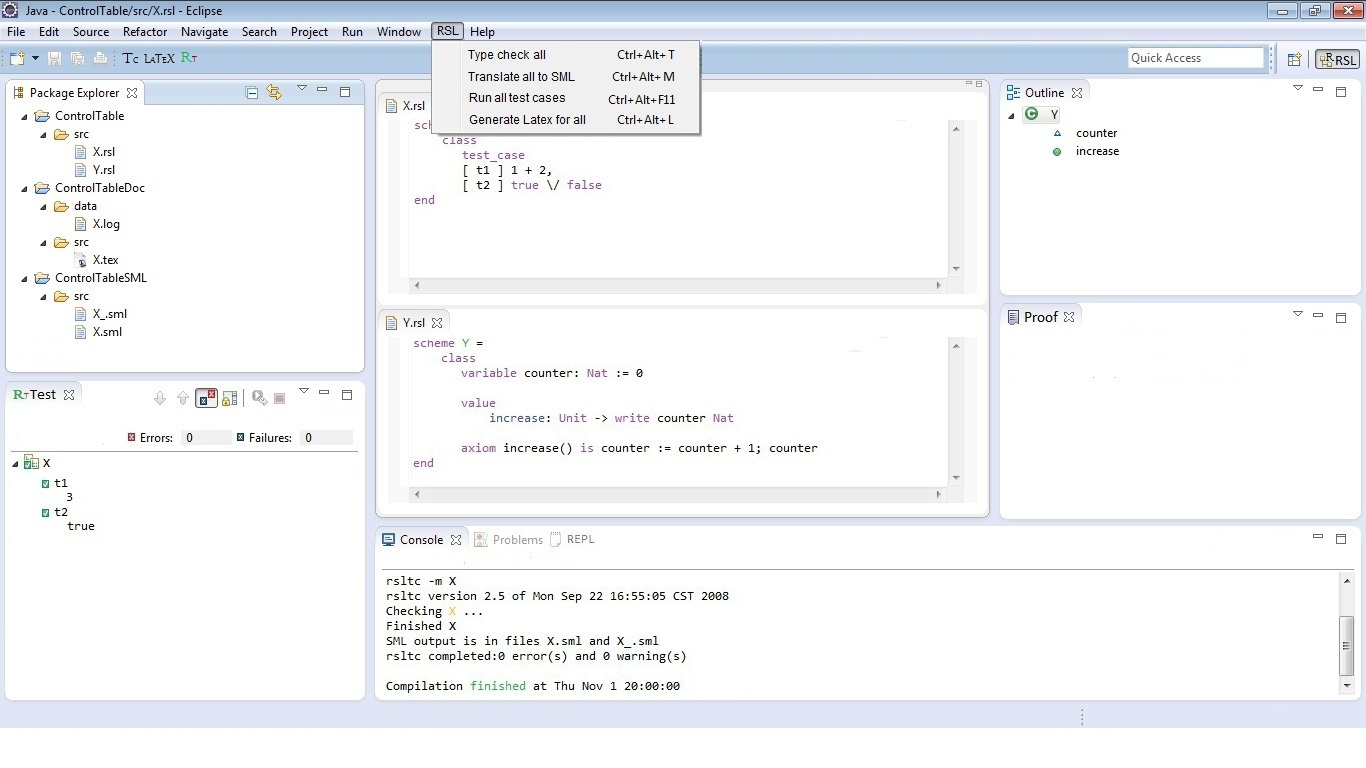
\includegraphics[width=2.5in]{RSLMenu.jpeg} 
% where an .eps filename suffix will be assumed under latex, 
% and a .pdf suffix will be assumed for pdflatex; or what has
% been declared via \DeclareGraphicsExtensions. 
\caption{Eclipse user interface displaying the RSL menu item} 
\label{UIMenu} 
\end{figure}

While the user interface is drawn, the requirements are documented in
EBON using \emph{scenario\_charts} elements. The beautiful part about
using EBON from the beginning is that it allows the requirements
specification to be captured using natural language. Therefore no
intermediate step is required between identifying the requirements and
documenting them. And to demonstrate it, this is how the
\emph{scenario\_charts} for the requirements presented in Figure
\ref{UIMenu}, looks like:

\begin{verbatim} 
	scenario_chart MENU 
	scenario "MENU1" 
	description "The
user can type check all RSL files in the workspace. Success or failure
messages will be displayed along with the list of errors in case of a
failure" 
	scenario "MENU2" 
	description "The user can translate to SML all RSL files in the
 workspace. Success or failure messages will be displayed along with
the list of errors in case of a failure" 
	scenario "MENU3" 
	description "The user can run all test cases in the workspace.
Success or failure messages will be displayed along with the list of
errors in case of a failure" 
	scenario "MENU4" 
	description "The user can generate Latex files for all files in
the workspace. Success or failure messages will be displayed along
with the list of errors in case of a failure" 
\end{verbatim}


% Events
%
\subsection{Events}
\emph{Incoming} events representing user actions and \emph{outgoing} events meant to inform the user.


% Components
%
\subsection{Components}
Major components captured in BON \emph{static\_diagram}s using \emph{cluster\_chart} and \emph{class}.


% Components communication
%
\subsection{Components communication}
Component interfaces added to the interface diagram using  \emph{feature}, \emph{require} and \emph{ensure}. This will later result in plug-in extensions and extension points.


Update scenarios with events.

% Code generation
%
\subsection{Code generation}
Beetlz generates the Java code from BON specification.

%------------------
% Conclusion
%------------------
\section{Conclusion}
In conclusion



% conference papers do not normally have an appendix


% use section* for acknowledgement
\section*{Acknowledgment}


The authors would like to thank...




% trigger a \newpage just before the given reference
% number - used to balance the columns on the last page
% adjust value as needed - may need to be readjusted if
% the document is modified later
%\IEEEtriggeratref{8}
% The "triggered" command can be changed if desired:
%\IEEEtriggercmd{\enlargethispage{-5in}}

% references section

% can use a bibliography generated by BibTeX as a .bbl file
% BibTeX documentation can be easily obtained at:
% http://www.ctan.org/tex-archive/biblio/bibtex/contrib/doc/
% The IEEEtran BibTeX style support page is at:
% http://www.michaelshell.org/tex/ieeetran/bibtex/
%\bibliographystyle{IEEEtran}
% argument is your BibTeX string definitions and bibliography database(s)
%\bibliography{IEEEabrv,../bib/paper}
%
% <OR> manually copy in the resultant .bbl file
% set second argument of \begin to the number of references
% (used to reserve space for the reference number labels box)
%
\begin{thebibliography}{1}

\bibitem{IEEEhowto:kopka}
H.~Kopka and P.~W. Daly, \emph{A Guide to \LaTeX}, 3rd~ed.\hskip 1em plus
 0.5em minus 0.4em\relax Harlow, England: Addison-Wesley, 1999.

\end{thebibliography}

% that's all folks
\end{document}


